\documentclass[a4paper, norsk, twoside, 10pt]{article}
%trennger en pakke med norske symboler
\usepackage{epsfig}
\usepackage{graphicx}
\usepackage{amsmath}
\usepackage{amsthm}
\usepackage{amssymb}
\usepackage[utf8]{inputenc}
\usepackage[a4]{}
\usepackage{float}
\usepackage{listings}
\usepackage[norsk]{babel}
\usepackage{color}
\usepackage{tikz}
\usetikzlibrary{arrows}

\newcommand{\RN}[1]{
  \textup{\uppercase\expandafter{\romannumeral#1}}%
}


\definecolor{mygreen}{RGB}{28,172,0} % color values Red, Green, Blue
\definecolor{mylilas}{RGB}{170,55,241}

\date{\today}
\title{Oblig1 \\ mat1120}
\author{Elsie Mestl}

\begin{document}
\maketitle
\begin{flushleft}

  \def\matrixP{
    \begin{bmatrix}
      1 & 0.7 & 0 & 0 & 0 \\
      0 & 0   & 0.5 & 0 & 0 \\
      0 & 0.3 & 0 & 0.65 & 0 \\
      0 & 0   & 0.5 & 0 & 0 \\
      0 & 0 & 0 & 0.35 & 1 \\
    \end{bmatrix}
  }

  \lstdefinestyle{custommat}{language=Matlab,%
    %basicstyle=\color{red},
    breaklines=true,%
    morekeywords={matlab2tikz},
    keywordstyle=\color{blue},%
    morekeywords=[2]{1}, keywordstyle=[2]{\color{black}},
    identifierstyle=\color{black},%
    stringstyle=\color{mylilas},
    commentstyle=\color{mygreen},%
    showstringspaces=false,%without this there will be a symbol in the places where there is a space
    frame = L,
    emph=[1]{for,end,break},emphstyle=[1]\color{red}, %some words to emphasise
    %emph=[2]{word1,word2}, emphstyle=[2]{style},
  }

  Generell antagelse for obligen er at når jeg har vist en matlabkommando, og dens respektive output en gang er det ikke nødvendig å gjøre dette senere i oppgaven. Da er det nok å si ``løst via matlab'' og så fortsette med oppgaven.

  \section*{Oppgave 1:}
  Matlabkoden:
  \lstinputlisting[style = custommat]{opgv1.m}
  \newpage
  
  Gir følgende output:
  \lstinputlisting[language = matlab, frame = L]{opgv1.out}
  \ \\
  \ \\
  Der hvor det i matlab-outputen viser P = ``matrise'' tilsvarer det $P^{n}$, n gitt linjen før. Vektroen som vises
  under tilsvarer sansylighetsfordelingen etter n kjøringer. Så sansynligheten for å gå fra $s_{4}$ til $s_{2}$ er posisjon 2 i vektoren
  og presisert i teksten under.


  \section*{Oppgave 2:}

  En matriser er A regulær hvis alle elementene i $A^{n}$ for alle n, er strengt større enn 0.
  \ \\
  Har
  \def\PI{
    \begin{bmatrix}
      0 & 0.7 & 0 & 0 & 0 \\
      0 & -1   & 0.5 & 0 & 0 \\
      0 & 0.3 & -1 & 0.65 & 0 \\
      0 & 0   & 0.5 & -1 & 0 \\
      0 & 0 & 0 & 0.35 & 0 \\
    \end{bmatrix}
  }


  \begin{align*}
    P -I &= \PI
  \end{align*}
  For å finne $Nul(P - I_{5})$ løser vi likingssettet:
  \[(P-I_{5}) \vec{x} = \vec{0} \]

  Som gir den utvidede matrisen:
  \[  \begin{bmatrix}
    0 & 0.7 & 0 & 0 & 0 & 0\\
    0 & -1   & 0.5 & 0 & 0 & 0\\
    0 & 0.3 & -1 & 0.65 & 0 & 0\\
    0 & 0   & 0.5 & -1 & 0 & 0\\
    0 & 0 & 0 & 0.35 & 0 & 0\\
  \end{bmatrix}\]

  Radreduserer denne, via matlab, og får:
  \lstinputlisting[style = custommat]{opgv2.m}
  \ \\
  \lstinputlisting[language = matlab, frame = L]{opgv2.out}

  Tar hensyn til de fri variablene og får følgende likningssytemer:
  \begin{align*}
    x_{2} = 0 \\
    x_{3} = 0 \\
    x_{4} = 0 \\
  \end{align*}

  Som kan skrives som:

  \[ \begin{bmatrix}
    x_{1} \\
    x_{2} \\
    x_{3} \\
    x_{4} \\
    x_{5} \\
  \end{bmatrix}
  =
  \begin{bmatrix}
    x_{1} \\
    0 \\
    0 \\
    0 \\
    x_{5}\\
  \end{bmatrix}
  = x_{1}
  \begin{bmatrix}
    1 \\
    0 \\
    0 \\
    0 \\
    0 \\
  \end{bmatrix}
  + x_{5}
  \begin{bmatrix}
    0 \\
    0 \\
    0 \\
    0 \\
    1 \\
  \end{bmatrix}
  = x_{1}\vec{u} + x_{5}\vec{v}
  \]


  Hvor $x_{1}$ og $x_{5}$ er fri variabler. Ser dermed at $\vec{u}$ og $\vec{v}$ spenner $Nul(P-I)$. De er også lineært uavhengige og dermed danner de også en basis for $Nul(P-I)$.
  \ \\ \ \\
  Siden summen av alle elementene i $\vec{u}$ og $\vec{v}$ summeres til 1 så er dette likevektsvektorer for matrisen P. Men siden $\vec{u}$ og $\vec{v}$ ikke er lineært uavhengige er finnes det heller ikke en unik (men to) likevektsvektorer, og P er dermed ikke en regulær matrise.
  \ \\ \ \\
  Ja, ser at $P^{n}$ ikke bare inneholder strengt positive, men også, null elementer, og kan dermed ikke være regulær.
\newpage
  \subsection*{Oppgave 3:}

  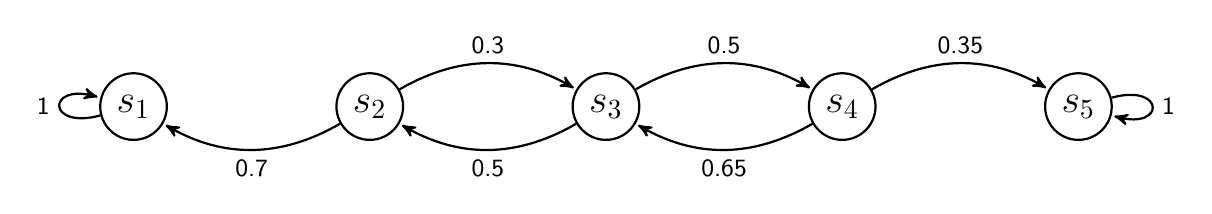
\begin{tikzpicture}[->,>=stealth',shorten >=1pt,auto,node distance=3cm,
      thick,main node/.style={circle,draw,font=\sffamily\Large\bfseries}]

    \node[main node] (1) {$s_{1}$};
    \node[main node] (2) [right of=1] {$s_{2}$};
    \node[main node] (3) [right of=2] {$s_{3}$};
    \node[main node] (4) [right of=3] {$s_{4}$};
    \node[main node] (5) [right of=4] {$s_{5}$};

    \path[every node/.style={font=\sffamily\small}]
    (1) edge [loop left] node {1} (1)
    (2) edge [bend left] node {0.3} (3)
        edge [bend left] node {0.7} (1)
    (3) edge [bend left] node {0.5} (2)
        edge [bend left] node {0.5} (4)
    (4) edge [bend left] node {0.65} (3)
        edge [bend left] node {0.35} (5)
    (5) edge [loop right] node {1} (5);
  \end{tikzpicture}


  \subsubsection*{a)}
  Har at klassene som utgjør S er:
  \begin{align*}
    K_{1} &= \{s_{1}\} \\
    K_{2} &= \{s_{2}, s_{3}, s_{4}\} \\
    K_{3} &= \{s_{5}\}\\
  \end{align*}

  Ser at både $K_{1}$ og $K_{3}$ er lukkede klasser, for de leder ingen noder som er utenfor sin egen klasse. Mens $K_{2}$ er en ikke lukket klasse pga $s_{2} \leadsto s_{1}$ og  $s_{4} \leadsto s_{5}$
  \ \\
  Siden $K_{1}$ og $K_{3}$ er lukkede og inneholder kun et element vil ethvert ``signal'' som kommer inn i disse klassene aldri komme ut. Ser dermed at $s_{1}$ og $s_{5}$ er absorberende.

  \subsubsection*{b)}

  Velger å se veldig generelt på denne oppgaven. \\
  La P være en regulær $n \times n$ matrise. Har at $P^{k}$ er strengt støre enn 0 for alle $k \in \mathbb{N}$. Elementene i P, $p_{ij}$, utgjør i hvilken grad tilstadene $s_{j} \leadsto s_{i}$ og siden  $p_{ij} \neq 0$ for alle $i,j$ har vi at tilstandene leder hverandre. Kan dermed si at alle elementene kommuniserer med hverandre. Og ugjør dermed en klasse.

  \subsection*{Oppgave 4:}

  Gjør samme regneoperasjon som i Oppgave 1. Men hvor startvektoren vår sitendenfor er:
  $\begin{bmatrix}
    0 \\
    1 \\
    0 \\
    0 \\
    0 \\
  \end{bmatrix}$
  og
    $\begin{bmatrix}
    0 \\
    0 \\
    1 \\
    0 \\
    0 \\
    \end{bmatrix}$.
  Som tilsvarer hendoldsvis $\vec{x_{2}}$ og $\vec{x_{3}}$\\
  $x_{2}^{K_{1}}$ tilsvarer da det 1. elementet fra vektoren som matrise-vektor multiplikasjonen utgjør: $P^{n}\cdot \vec{x_{2}}$ \\$x_{2}^{K_{3}}$ utgjør det 5 elementet i den samme vektoren. \\ \ \\
  Det tilsvarende stemmer også for $x_{3}^{K_{1}}$ og $x_{3}^{K_{3}}$ men hvor starttilstanden istedenfor er $\vec{x_{3}}$

  Får:
  \[ P^{100}\cdot \vec{x_{2}} = \begin{bmatrix}
    0.9 \\
    0 \\
    0 \\
    0 \\
    0.1 \\
  \end{bmatrix}, \quad
  P^{100}\cdot \vec{x_{3}} = \begin{bmatrix}
    \frac{2}{3} \\
    0 \\
    0 \\
    0 \\
    \frac{1}{3} \\
  \end{bmatrix}
  \]
  Altså er:
  \begin{align*} x_{2}^{K_{1}} &= 0.9 \quad &x_{3}^{K_{1}} = \frac{2}{3} \\
    x_{2}^{K_{3}} &= 0.1 \quad &x_{3}^{K_{3}} = \frac{1}{3} \\
  \end{align*}


  \subsection*{Oppgave 5:}

  \def\matrixPgen{
    \begin{bmatrix}
      1 & p_{2} & 0 & 0 & 0 \\
      0 & 0   & p_{3} & 0 & 0 \\
      0 & q_{2} & 0 & p_{4} & 0 \\
      0 & 0   & q_{3} & 0 & 0 \\
      0 & 0 & 0 & q_{4} & 1 \\
   \end{bmatrix}
  }
   \[P = \matrixPgen \]
   \subsubsection*{a)}
   Tilstanden $s_{1}$ tilsvarer kolonne 1 i $P$. Og ser at det kun er det første elementet som har en verdi, verdien 1. Altså vil alt som kommer inn i $s_{1}$ loope tilbake til seg selv. Tilstanden kommuniserer heller ikke med noen andre tilstander så $\{s_{1}\}$ utgjør en lukket klasse, og $s_{1}$ er dermed absorberende.\\
   \ \\
   Det samme ser vi for tilstand $s_{5}$, kommuniserer bare med seg selv. Og leder ingen andre tilstander. Altså er også $s_{5}$ absorberende.


   \subsubsection*{b)}
   $x_{1} = 1$ fordi $s_{1}$ er absorberende og $x_{1}$ er et element i $s_{1}$ \\
   $x_{5} = 0$ fordi $s_{5}$ er absorberende og $x_{5}$ er et element i denne tilstande. Kan dermed ikke ``unslippe'' og gå over til en annen tilstand. \\
   \ \\
   Har gitt at:
   \[x_{j}^{K} = \sum_{i = 1}^{n} p_{ij}x_{i}^{K}\]\\

   Skriver vi ut  likningssettet for n = 1 til n = 5 vha likningen og det beskrevet over får vi:
   \begin{align*}
     x_{1}^{2} &= 1 \\
     x_{2}^{2} &= p_{12}x_{1}^{2} + p_{22}x_{2}^{2} + p_{32}x_{3}^{2} + p_{42}x_{4}^{2} + p_{52}x_{5}^{2} \\
     x_{3}^{2} &= p_{13}x_{1}^{2} + p_{23}x_{2}^{2} + p_{33}x_{3}^{2} + p_{43}x_{4}^{2} + p_{53}x_{5}^{2} \\
     x_{4}^{2} &= p_{14}x_{1}^{2} + p_{24}x_{2}^{2} + p_{34}x_{3}^{2} + p_{44}x_{4}^{2} + p_{54}x_{5}^{2}\\
     x_{5}^{2} &= 0 \\
   \end{align*}
   Som vi leser ut av matrisen $P$ og ser at blir:

   \begin{align*}
     x_{1}^{2} &= 1 \\
     x_{2}^{2} &= p_{2} + q_{2}x_{3}^{2} \\
     x_{3}^{2} &= p_{3}x_{2}^{2} + q_{3}x_{4}^{2}\\
     x_{4}^{2} &= p_{4}x_{3}^{2}\\
     x_{5}^{2} &= 0 \\
   \end{align*}   

   Flytter vi $x$ene over på en side får vi likningene:
   \begin{align*}
     x_{2}^{2}  - q_{2}x_{3}^{2} &= p_{2}\\
     x_{3}^{2} - p_{3}x_{2}^{2} - q_{3}x_{4}^{2}&= 0\\
     x_{4}^{2} - p_{4}x_{3}^{2} &= 0\\
   \end{align*}   
   
   Setter inn i en matrise får vi følgende:

   \[\begin{bmatrix}
   1 & - q_{2} & 0 & p_{2}\\
   -p_{3} & 1 & -q_{3} & 0 \\
   0 & -p_{4} & 1 & 0 \\
   \end{bmatrix}\]

   Ser at dette er matrise A, og har at for $\vec{y} = (x_{2}, x_{3}, x_{4})$ vil svaret $\vec{b}$ tilsvare høyre kolonne, altså $(p_{2}, 0, 0)$



   \subsection*{c}
   En matrise er definert som øvre trianguler dersom alle elementene under diagonalen er 0. \\

   Utfører operasjonene som ville blitt brukt for å lage pivot søyler av de to første søylene i A, altså: \\ \ \\
   Legger til $p_{3}$Rad$\RN{1}$ til Rad$\RN{2}$. Da er de to elementene under diagonalen i kolonne en 0.\\
   Legger til $p_{4}$Rad$\RN{2}$ til Rad$\RN{3}$. Det fjerner det tredje elementet som ligger i kolonne 2.
   \\
   Altså er A radredusert til en øvre diagonal matrise.
   
  \end{flushleft}
\end{document}
